\documentclass{beamer}
\usepackage[utf8]{inputenc}

\usetheme{Copenhagen}
%color themes: default, beaver, beetle, seahorse, wolverine
\usecolortheme{default}
 
 
%Information to be included in the title page:
\title{Bastion The Sentinel}
\author{Park Cleaner Robot}
\logo{
\includegraphics[height=1.5cm]{bastion}}
\institute{Istanbul Bilgi University}
\date{\today}
 
 
\begin{document}
 % Giriş sayfasını yazdır
 \frame{\titlepage}
 
 %scope slaytı
 \begin{frame}
  \frametitle{SCOPE}
  \begin{itemize}
   \item Consuming essential for humans
   \item It leads to pollution
   \item Our main goal is separating and recycling the garbages
  \end{itemize}
 \end{frame}

 %device functionality slaytı
 \begin{frame}
  \frametitle{DEVICE FUNCTIONALITY}
  \begin{itemize}
   \item Bastion The Sentinel will be a multi-tasking that has two main parts.
   \begin{itemize}
    \item Movement controls
    \item Robotic arm controls
   \end{itemize}
   \item Designed as a semi-autonomous robot
   \item Robotic arm uses image processing to collect garbages
   \begin{itemize}
    \item Image recognization by color difference
    \item Image recognization by shape
   \end{itemize}
   \item Operator takes control in emergency situations
  \end{itemize}
 \end{frame}

 %device functionality slaytı
 \begin{frame}
  \frametitle{DEVICE FUNCTIONALITY}
  \begin{itemize}
   \item It has resizable box
   \item It is accelerating from front wheels
   \item To increase the maneuver ability, we placed steering wheels to the back
   \item It uses:
   \begin{itemize}
    \item Proximity sensor
    \item Depth sensor
    \item Light sensor
    \item Cameras
   \end{itemize}
  \end{itemize}
 \end{frame}

 %overall design scheme
 \begin{frame}
  \frametitle{OVERALL DESIGN SCHEME}
  \begin{figure}[h]
   \begin{center}
    \includegraphics[scale=0.38]{block_diagram}
    \caption{Block diagram of the system}
   \end{center}
  \end{figure}
 \end{frame}
 
 %details of design
 \begin{frame}
  \frametitle{DESIGN AND DETAILS}
  \begin{itemize}
   \item Input Block
   \begin{itemize}
    \item Cameras
   \end{itemize}
   \item Control Block
   \item Output Block
   \item Communication Block
  \end{itemize}
 \end{frame}

 %input block
 \begin{frame}
  \frametitle{Input Block}
  \begin{itemize}
    \item \textbf{Bastion The Sentinel}'s robotic arm divided by three joints and has one gripper.
    \item Robotic arm can rotate 360$^{\circ}$ and it can be collapsed to minimize the area. Also the gripper part will 
    have the ability to rotate up to 180$^{\circ}$.
    \item Garbage detection is reinforced by proximity sensor. It will provide information about whether there is an object around 
    of the robot.
    \item Depth sensor will be used to verify incoming data's from proximity sensor. If they match the robotic arm will start the 
    collecting process.
  \end{itemize}
 \end{frame}
 
 %cameras
  \begin{frame}
  \frametitle{Input Block}
  Cameras:\\
  \bigskip
  \begin{itemize}
    \item There are 3 CMOS Camera Sensor
    \item Two of them will be used as both depth sensor and vision camera
    \item We will switch between two mods:
    \begin{itemize}
     \item Depth mode
     \item Vision mode
    \end{itemize}
    \item Third camera will help us to put garbages in the box
  \end{itemize}
 \end{frame}
 
 %control block
 \begin{frame}
  \frametitle{Control Block}
  \begin{flushleft}
     \begin{figure}[h!]
      \begin{center}
       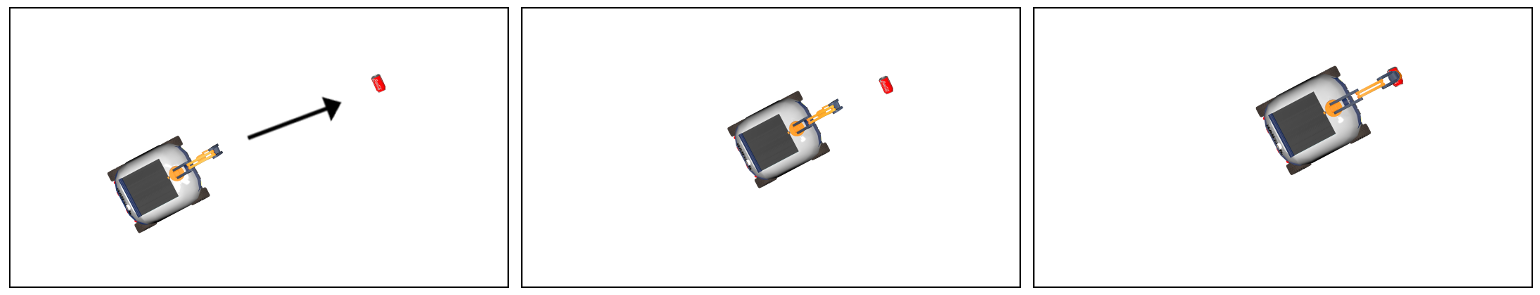
\includegraphics[scale=0.2]{3frame}
       \caption{\textbf{Bastion The Sentinel} is approaching to an object.}
      \end{center}
     \end{figure}
     In this block, Arduino (and Raspberry Pi) will manage the wheel system. It gives impulse to front wheels while it only 
     rotates from back wheels. Two motor shields will drive four wheels.
    \end{flushleft}
 \end{frame}

 % output block
 \begin{frame}
  \frametitle{Output Block}
  \begin{figure}[h]
      \begin{center}
       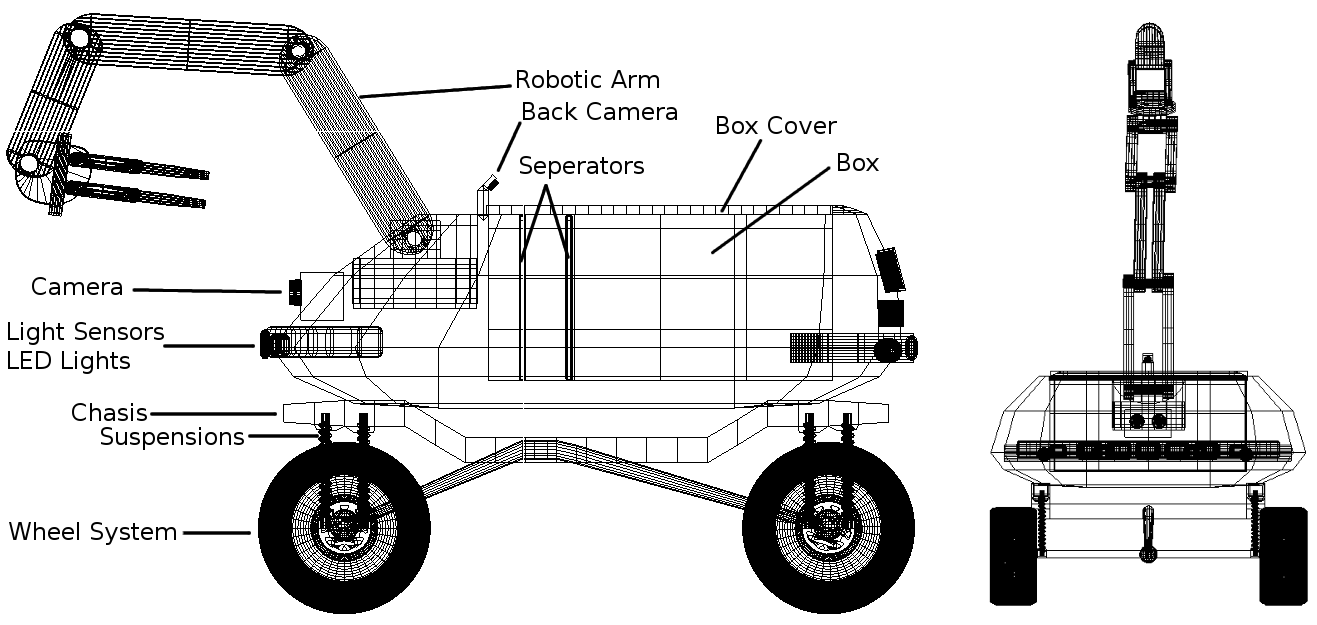
\includegraphics[scale=0.3]{skeleton_detailed}
      \end{center}
     \end{figure}
 \end{frame}
 
 %communication block
 \begin{frame}
  \frametitle{Communication Block}
  \begin{itemize}
   \item Wireless connection on Raspberry Pi 3
   \item Sensor information will be processed on the robot and will be sent to user
   \item Video data will be processed on user side
   \item Simultaneous data transmission
  \end{itemize}
 \end{frame}

 %time table
 \begin{frame}
  \frametitle{TIME TABLE AND WORK SCHEDULE}
  \begin{figure}[h]
    \begin{center}
      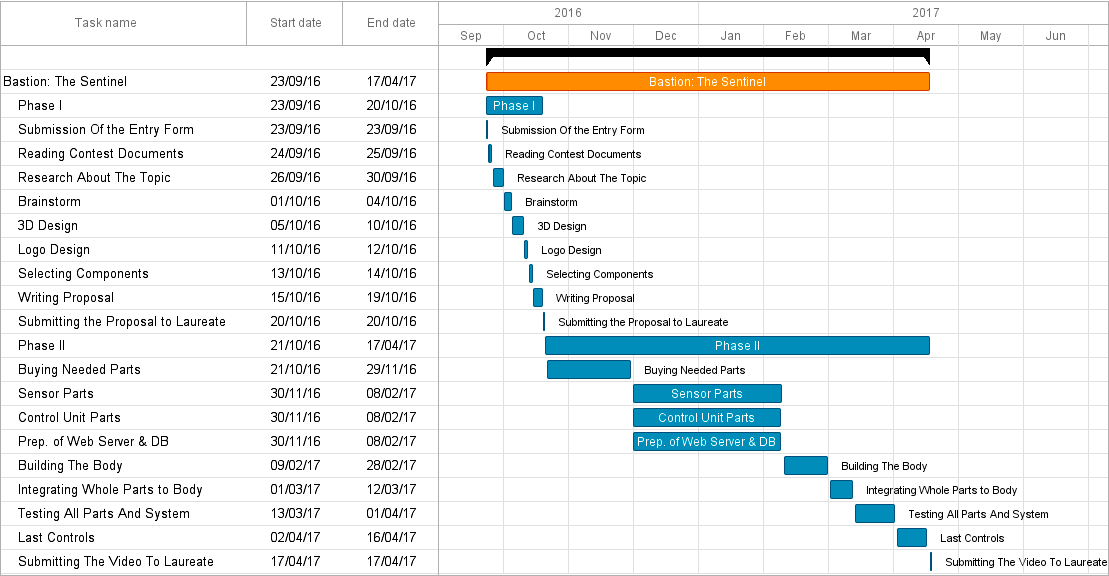
\includegraphics[scale=0.27]{time_schedule}
      \caption{Phase I and Phase II in details}
    \end{center}
   \end{figure}
 \end{frame}

 %cad design
 \begin{frame}
  \frametitle{CAD DESIGN AND DEVICE DIMENSIONS}
  \begin{figure}[h!]
   \begin{center}
    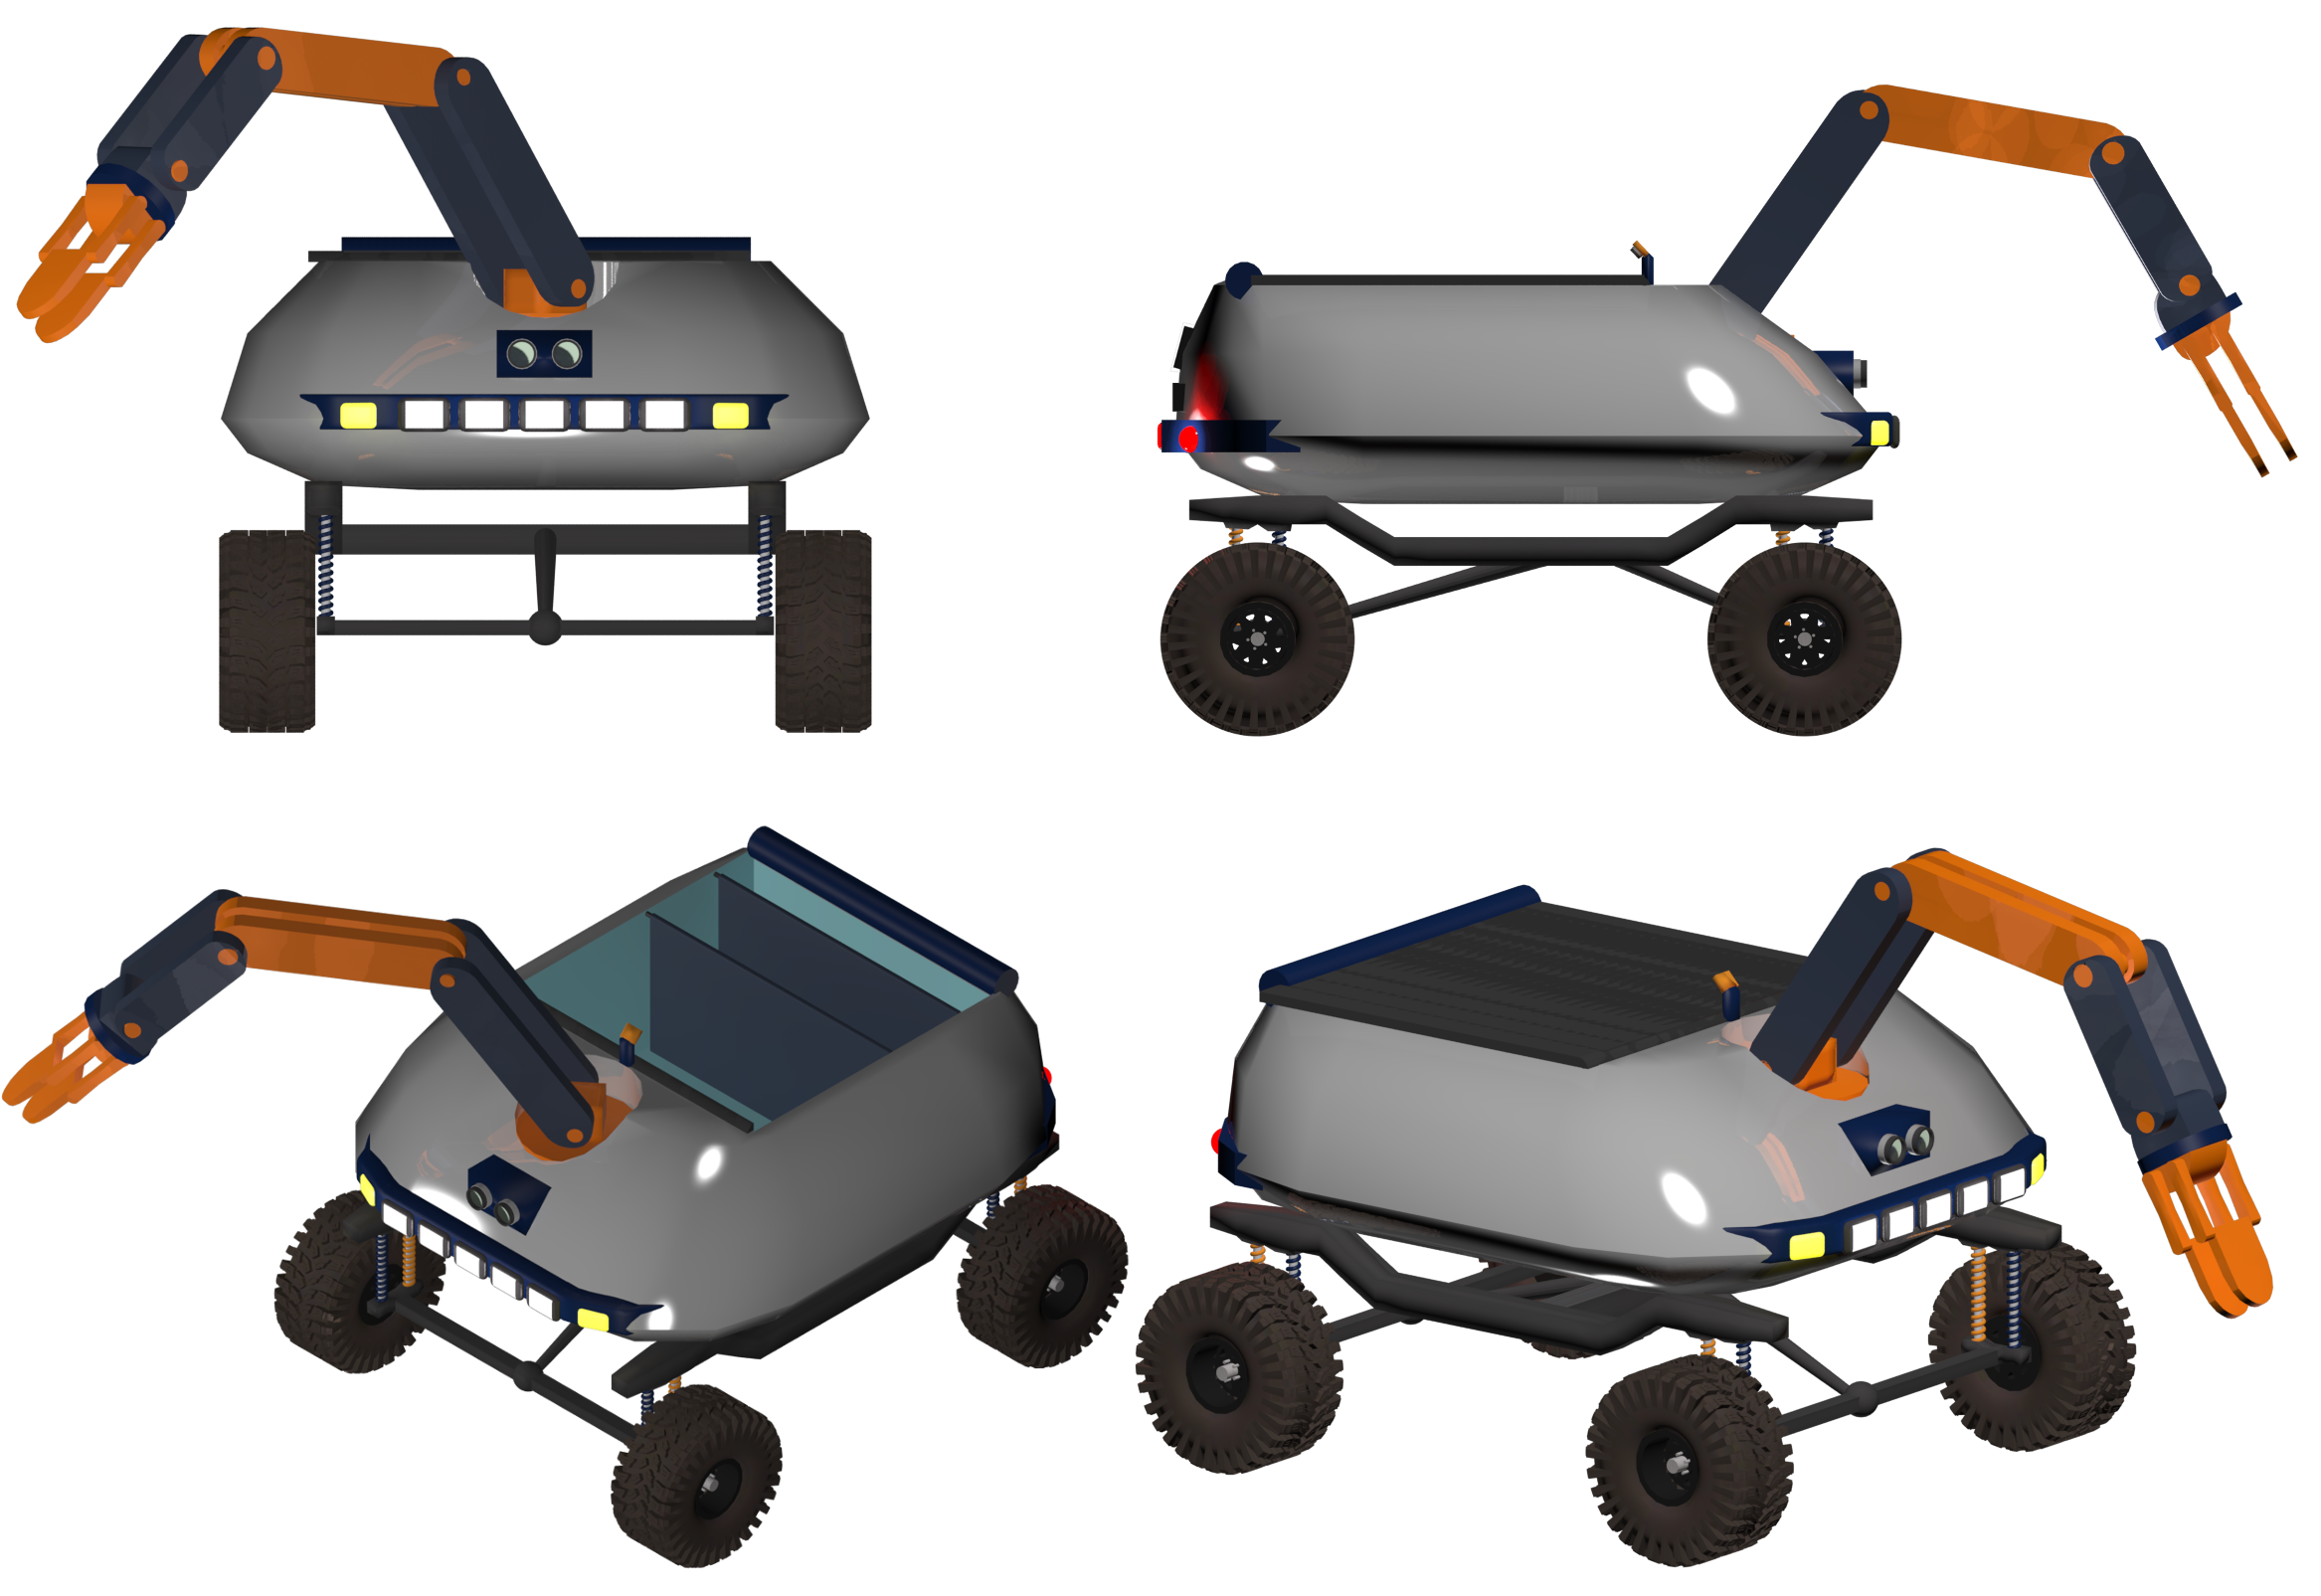
\includegraphics[scale=0.12]{cad_design}
    \caption{CAD design, Approximate Dimensions: Length=50cm Width=45cm Height=40cm}
   \end{center}
  \end{figure}
 \end{frame}
 
  %budget
 \begin{frame}
  \frametitle{BUDGET}
  \begin{figure}[h!]
   \begin{center}
    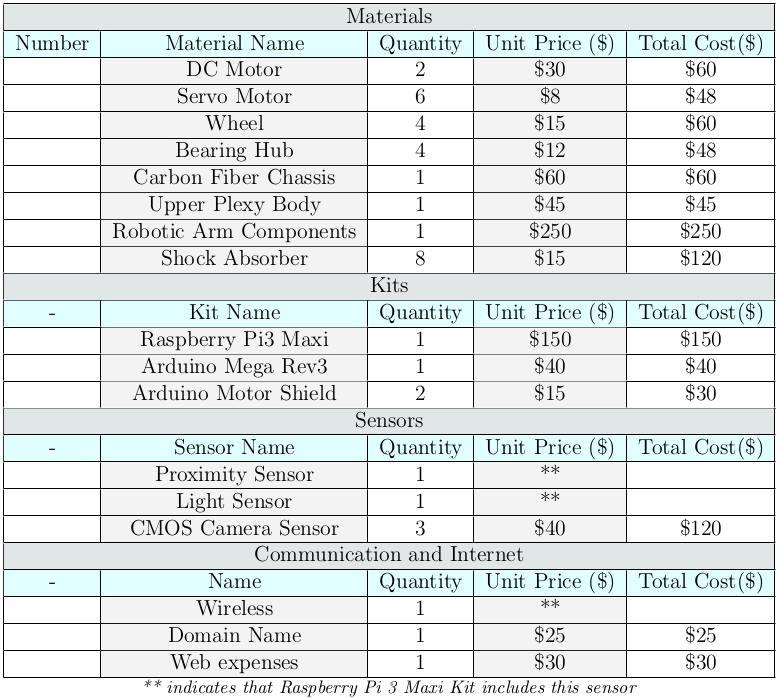
\includegraphics[scale=0.3]{budget}
   \end{center}
  \end{figure}
 \end{frame}
 
 %Safety and Environmental Sustainability
 \begin{frame}
  \frametitle{SAFETY AND ENVIRONMENTAL SUSTAINABILITY}
  \begin{itemize}
   \item Robot operates in a semi-autonomous way
   \item Robot will interact with the environment
   \item It leads some dangerous situations
   \item In this type of situations operator will take the control
  \end{itemize}
 \end{frame}

 %Business plan
 \begin{frame}
  \frametitle{BUSINESS PLAN}
  \begin{itemize}
   \item In Turkey, pollution rates are higher than other countries
   \item There is no proper way to solve this problem
   \item The purpose of creating this robot is to protect the nature and speed up the recycling process
   \item It takes so many years for some materials to dissolve in nature
   \item \%75 of garbages are recyclable but \%30 percent of it used used in recycling process
   \item Someone should step up and do something about it
   \item While we are making the nature cleaner, also we are aiming to build a robot which has recyclable parts as much as possible.
  \end{itemize}
 \end{frame}
 
\end{document}